\section{Element Deletion}

Elements can easily be deleted using the delete button found in the toolbar. You can also press delete with the item you want to delete selected. Following is a simple walk through for deleting an element.

First, choose the type of the element you wish to delete. This can be either Projects, Teams, People, Skills, Releases, Backlogs, Stories or Sprints and select it in the Display Choice Picker (circled below).

\begin{figure}[H]
\centering
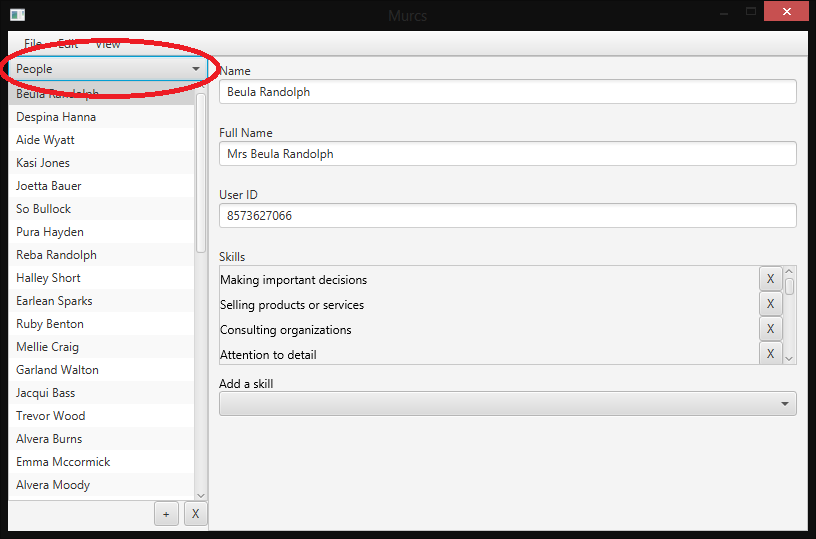
\includegraphics[width=\textwidth]{images/screenshots/deletion1.PNG}
\caption{The Display Choice Picker}
\label{fig:new_project}
\end{figure}

In our case, we've chosen to delete a person named Dion Vader. The next step is to select this person and press the delete button (circled below).

\begin{figure}[H]
\centering
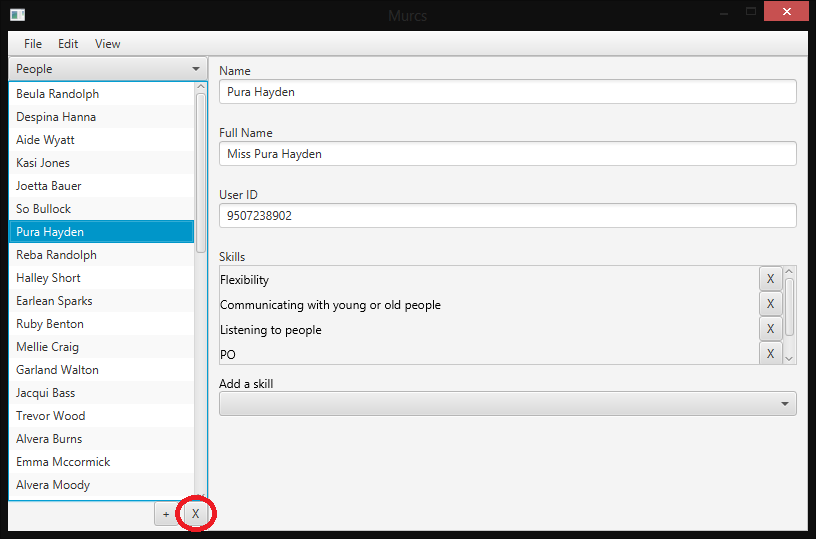
\includegraphics[width=\textwidth]{images/screenshots/deletion2.PNG}
\caption{The Delete Button}
\label{fig:new_project}
\end{figure}

The final step is to confirmation. You will be a presented with a message asking you if you are really sure you want to go through with a deletion along with a list of places that the element you are deleting is used. Press the 'Yes' button (circled) to go through with the deletion. If you've changed your mind you can click the 'No' button. 

\begin{figure}[H]
\centering
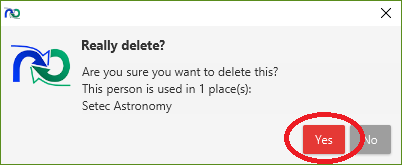
\includegraphics[width=\textwidth]{images/screenshots/deletion3.PNG}
\caption{The Confirmation Dialog. It seems Dion is part of a team named 'Setec Astronomy'}
\label{fig:new_project}
\end{figure}

Deleting Dion also removes him from anywhere else he may be used, so be careful!

If you've deleted something by mistake, don't worry! Deletions can be undone. Phew.